%% COSC 520 Assignment 2 - Mergeable heaps: binomial, Fibonacci and pairing heaps
%% ACM Small format with the ACM, journal and copyright information removed.
%% Compile with pdfLaTeX + BibTeX (Overleaf default).

\documentclass[acmsmall,nonacm]{acmart}

\setcopyright{none}
\settopmatter{printacmref=false}
\renewcommand\footnotetextcopyrightpermission[1]{}
\pagestyle{plain}

\newcommand{\us}{\,$\mu$s}
\newcommand{\code}[1]{\texttt{#1}}

\begin{document}

\title{Mergeable Heaps in Theory and Practice: Binomial, Fibonacci and Pairing Heaps Compared}
\subtitle{COSC 520 Assignment 2 --- Student number 84298512}

\author{Ahmed Elgazwy}
\email{ahmed.elgazwy@ubc.ca}
\affiliation{%
  \institution{University of British Columbia}
  \city{Kelowna}
  \state{British Columbia}
  \country{Canada}}

\begin{abstract}
We implement three mergeable priority queues from scratch in Python (the
binomial, Fibonacci and pairing heaps) behind one interface, analyse the
amortized cost of their operations, and benchmark them on $10^7$ random keys and
on Dijkstra's algorithm over a graph with $10^6$ vertices and $10^7$ edges. The
measured growth rates confirm the analysis: inserts take constant time, the
first extract-min after $n$ inserts costs $\Theta(n)$ for the two lazy heaps
(8.1\,s for the Fibonacci heap at $n = 10^7$, against 0.04\,ms for the binomial
heap), and a decrease-key to a new minimum costs 1.9--2.4\us{} in the lazy heaps
against 9.7\us{} in the binomial heap. The textbook ranking for Dijkstra's
algorithm, however, is reversed. The Fibonacci heap has the best bound,
$O(E + V\log V)$, yet it is the slowest (37.5\,s, against 26.8\,s for the
pairing heap): only 0.99 decrease-keys per vertex occur, and its extract-min is
2.4 times slower than the pairing heap's. The pairing heap is the fastest heap
in steady state and the smallest, at 102 bytes per item.
\end{abstract}

\keywords{priority queues, mergeable heaps, Fibonacci heap, pairing heap, binomial heap, amortized analysis, Dijkstra's algorithm}

\maketitle

%% ---------------------------------------------------------------------------
\section{Introduction}

A priority queue stores items with keys and repeatedly hands out the one with
the smallest key. Two further operations distinguish the \emph{mergeable heaps}
studied here: \code{decrease\_key}, which lowers the key of an item already in
the queue, and \code{merge}, which combines two queues. Dijkstra's
shortest-path algorithm~\cite{dijkstra1959} calls \code{decrease\_key} whenever
it finds a shorter path, and Fibonacci heaps were designed to make that call
$O(1)$ amortized, which gives Dijkstra's algorithm its best known bound,
$O(E + V \log V)$~\cite{fredman1987}. Experimental studies, however, report
that the simpler pairing heap~\cite{fredman1986} is efficient in
practice~\cite{stasko1987} and faster than the Fibonacci
heap~\cite{larkin2014}, even though its analysis is still
open~\cite{fredman1999,pettie2005}.

This report asks whether the analysis predicts the measured behaviour of the
three heaps, implemented by hand in Python, at ten million items. It makes four
contributions:
\begin{itemize}
  \item implementations of the binomial, Fibonacci and pairing heaps behind one handle-based interface, with Dijkstra's algorithm on top and 428 unit tests;
  \item a complexity analysis of every operation, with the potential functions and bounds it rests on (Section~\ref{sec:complexity});
  \item a benchmark on a published dataset of $10^7$ keys and a $10^7$-edge graph (Sections~\ref{sec:setup}--\ref{sec:results});
  \item an explanation of where the measurements follow the analysis and where they do not (Section~\ref{sec:discussion}).
\end{itemize}

\noindent\textbf{Code:} \url{https://github.com/ahmedelgazwy/Advanced_DS_assignment_2}\\
\textbf{Dataset:} \url{https://github.com/ahmedelgazwy/Advanced_DS_assignment_2/releases/tag/dataset-v1}

%% ---------------------------------------------------------------------------
\section{Why These Structures}
\label{sec:why}

I selected these heaps because I wanted to see which one would perform best in
a realistic scenario, finding shortest paths with Dijkstra's algorithm, and
whether the Fibonacci heap, which has the best theoretical bounds, would also
be the fastest in practice. I was also interested in how differently they are
built: the binomial heap uses a series of trees, while the pairing heap uses a
single tree, and I wanted to see whether this leads to a tradeoff between time
and space. More generally, the idea of using trees to build a priority queue
was interesting to me. In the end there was no tradeoff: the single-tree
pairing heap was both the fastest and the smallest of the three.

%% ---------------------------------------------------------------------------
\section{The Three Heaps and Their Applications}
\label{sec:structures}

All three heaps store \code{(key, value)} items and implement one interface:
\code{insert} returns a \emph{handle} to the new item, and the caller later
passes that handle to \code{decrease\_key} or \code{delete}. The interface also
offers \code{find\_min}, \code{extract\_min} and a destructive \code{merge}.
No library priority queue is used (no \code{heapq}, no \code{queue}), and every
algorithm is iterative: a pairing heap after $n$ sorted inserts is $n$ levels
deep, far beyond Python's recursion limit of 1,000.

\textbf{Binomial heap}~\cite{vuillemin1978,brown1978}. A binomial tree $B_k$
consists of two $B_{k-1}$ trees, one linked below the other's root. A binomial
heap is a list of heap-ordered binomial trees with at most one tree of each
order, so the orders present are the 1-bits of $n$: thirteen items form $B_3$,
$B_2$ and $B_0$. Merging two heaps works like binary addition, where linking two
trees of equal order is the carry~\cite[Problem~19-2]{cormen2009}. We keep a
pointer to the minimum root, so \code{find\_min} is $O(1)$.
\code{decrease\_key} moves the item up its tree. The textbook version swaps
keys between a node and its parent~\cite[ch.~19]{cormen2001}, which would leave
a caller's handle pointing at the wrong item. We therefore store each item in a
separate object that points back to its node, and swap whole items.

\textbf{Fibonacci heap}~\cite{fredman1987}. A collection of heap-ordered trees
whose roots form a circular doubly linked list~\cite[ch.~19]{cormen2009}. The
structure is \emph{lazy}: \code{insert} and \code{merge} only splice lists, and
all tidying is left to \code{extract\_min}, which \emph{consolidates} the roots
until no two have the same degree. \code{decrease\_key} cuts a node whose key
became smaller than its parent's and moves it to the root list. A node that
loses a second child is cut as well (a \emph{cascading cut}); a mark bit records
the first loss.

\textbf{Pairing heap}~\cite{fredman1986}. A single heap-ordered multiway tree.
Its only primitive, \emph{link}, makes the larger of two roots the leftmost
child of the smaller. \code{insert}, \code{merge} and \code{decrease\_key} are
one link each (\code{decrease\_key} first cuts the node's subtree out). All
restructuring happens in \code{extract\_min}, which combines the root's
children by \emph{two-pass pairing}: it links them in pairs from left to right,
then links the results one by one from right to left. Each node keeps a
pointer to its left sibling (or its parent), so a subtree is cut out in $O(1)$.

\textbf{Applications.} Mergeable heaps with \code{decrease\_key} are the
priority queues of Dijkstra's shortest-path algorithm and Prim's
minimum-spanning-tree algorithm, the applications for which Fibonacci heaps
were introduced~\cite{fredman1987}. More generally they serve any system that
schedules work by priority and must re-prioritize waiting items, such as
event-driven simulators and job schedulers, and \code{merge} combines the
queues of two such schedulers in $O(1)$ or $O(\log n)$ time. All three heaps
are available in Boost.Heap, with handles for updating keys~\cite{boostheap},
and the pairing heap is the default of GCC's policy-based
\code{priority\_queue}~\cite{gccpbds}.

%% ---------------------------------------------------------------------------
\section{Complexity Analysis}
\label{sec:complexity}

Let $n$ be the number of items, $D(n)$ the largest degree of a node, $t(H)$ the
number of trees in the root list, $m(H)$ the number of marked nodes,
$\varphi = (1+\sqrt5)/2$ and $F_k$ the $k$-th Fibonacci number. For Dijkstra's
algorithm, $V$ and $E$ are the numbers of vertices and edges. An
\emph{amortized} bound holds for the total cost of any sequence of operations
divided by its length; all three analyses use the potential
method~\cite[\S{}17.3]{cormen2009}. Table~\ref{tab:complexity} summarizes the
bounds.

\begin{table}[t]
\caption{Time and space complexity. Binomial-heap bounds are worst case per operation; the other two are amortized, and a single extract-min of a lazy heap can cost $O(n)$.}
\label{tab:complexity}
\small
\begin{tabular}{@{}llll@{}}
\toprule
Operation & Binomial & Fibonacci (amortized) & Pairing (amortized) \\
\midrule
insert & $O(\log n)$; $O(1)$ amortized & $O(1)$ & $O(1)$~\cite{iacono2000} \\
find-min & $O(1)$ (min pointer) & $O(1)$ & $O(1)$ \\
extract-min, delete & $O(\log n)$ & $O(\log n)$ & $O(\log n)$~\cite{fredman1986} \\
decrease-key & $O(\log n)$ & $O(1)$ & $\Omega(\log\log n)$~\cite{fredman1999}, $O(2^{2\sqrt{\log\log n}})$~\cite{pettie2005} \\
merge & $O(\log n)$ & $O(1)$ & $O(1)$~\cite{iacono2000} \\
space & $\Theta(n)$ & $\Theta(n)$ & $\Theta(n)$ \\
Dijkstra & $O((V+E)\log V)$ & $O(E + V\log V)$ & $O((V+E)\log V)$ \\
\bottomrule
\end{tabular}
\end{table}

\textbf{Binomial heap.} By induction, $B_k$ has $2^k$ nodes and height $k$,
and its root has degree $k$~\cite[Lemma~19.1]{cormen2001}. Since the orders
present are the 1-bits of $n$, a heap has at most $\lfloor\log_2 n\rfloor + 1$
trees, and every node has degree at most $\log_2 n$. Union walks the two root
lists once, extract-min unions the $\le \log_2 n$ children of the removed root
back in, and decrease-key climbs a path no longer than a tree's height: each is
$O(\log n)$. An insert is a binary-counter increment. With the potential
$\Phi = t(H)$, an insert that performs $c$ carries costs $1+c$ and changes
$\Phi$ by $1-c$, so its amortized cost is $(1+c)+(1-c) = 2 = O(1)$, although a
single insert can still cost $\Theta(\log n)$.

\textbf{Fibonacci heap.} With $\Phi(H) = t(H) + 2\,m(H)$~\cite{fredman1987},
insert raises $\Phi$ by 1 and merge leaves it unchanged, so both are $O(1)$.
Extract-min costs $O(D(n) + t(H))$ but leaves at most $D(n)+1$ roots, so the
drop in potential pays for the $t(H)$ term and the amortized cost is
$O(D(n))$. A decrease-key that triggers $c$ cascading cuts costs $O(c)$ and
changes $\Phi$ by at most $(t+c) + 2(m-c+2) - (t+2m) = 4-c$: amortized $O(1)$.
The bound on $D(n)$ gives the structure its name: the $i$-th child of a node
has degree at least $i-2$, so a node of degree $k$ roots at least
$F_{k+2} \ge \varphi^k$ nodes, and $D(n) \le \lfloor\log_\varphi n\rfloor \approx
1.44\log_2 n$~\cite[Lemma~19.4, Cor.~19.5]{cormen2009}. Our consolidation table
uses the exact bound $\max\{k : F_{k+2} \le n\}$ in integer arithmetic (33 at
$n = 10^7$). Amortization hides spikes: right after $n$ inserts, $t(H) = n$ and
the first extract-min does $\Theta(n)$ work.

\textbf{Pairing heap.} Fredman et al.\ proved $O(\log n)$ amortized time for
every operation~\cite{fredman1986}, and Iacono reduced insert and merge to
$O(1)$~\cite{iacono2000}. Decrease-key is provably \emph{not} $O(1)$: it needs
$\Omega(\log\log n)$ amortized time~\cite{fredman1999,iacono2014}, and the best
upper bound is $O(2^{2\sqrt{\log\log n}})$~\cite{pettie2005}. These bounds come
from different analyses and the exact cost is open. In practice the gap is
academic: $2^{2\sqrt{\log_2\log_2 n}}$ only falls below $\log_2 n$ for
$n > 2^{16}$, and at $n = 10^7$ the two are 19.2 and 23.3.

\textbf{Space.} All three heaps use $\Theta(n)$ space, one node per item, but
their nodes differ: 5 fields for the binomial heap (plus a 3-field item object
for handles), 8 for the Fibonacci heap and 5 for the pairing heap. With
\code{\_\_slots\_\_}, CPython 3.10 objects with 3, 5 and 8 fields take 56, 72 and
96 bytes, and a random 31-bit key about 30 bytes, which predicts 158, 126 and
102 bytes per item.

\textbf{Dijkstra's algorithm} performs at most $V$ inserts and extract-mins and
at most $E$ decrease-keys, which gives the bounds in
Table~\ref{tab:complexity}. The $E$ term only matters if many relaxations
actually lower a key. If the lengths of the edges entering each vertex are
independent and identically distributed, the expected number of decrease-keys
is only $O(V\log(1 + E/V))$~\cite{goldberg1996}.

%% ---------------------------------------------------------------------------
\section{Experimental Setup}
\label{sec:setup}

\textbf{Machine.} Intel Core i7-11800H (8 cores, 24\,MB L3 cache), 16\,GiB
RAM, Windows 11 (build 26200), CPython 3.10.2. The full benchmark ran in 13
minutes.

\textbf{Data.} The dataset has two parts:
\begin{itemize}
  \item $10^7$ keys drawn uniformly from $[0, 2^{31})$ by a seeded generator. The first $n$ keys form the dataset of size $n$, so one file serves every size.
  \item A directed graph with $V = 10^6$ vertices and $E = 10^7$ edges with weights uniform in $[1, 1000]$. Its first $V-1$ edges form a random Hamiltonian path from vertex 0, so every vertex is reachable from the source. The remaining edges join random pairs of distinct vertices.
\end{itemize}
Both files are published with SHA-256 checksums, and regenerating them
reproduces the same bytes. Random keys are the standard average case. The
sparse graph ($E = 10V$) is the regime in which the Fibonacci heap's
$O(E + V\log V)$ bound should help most.

\textbf{Workloads.} For $n$ on a 1--2--5 ladder from $10^3$ to $10^7$, each
heap is built as two heaps of $n/2$ keys that are then merged. We then time,
with $K = \min(10^5, n/10)$:
\begin{itemize}
  \item the first extract-min;
  \item a warm-up batch of $K$ extract-mins, kept apart from a steady-state batch of $K$ more;
  \item $K$ decrease-keys whose new keys are drawn between the current minimum and the old key, as in Dijkstra's algorithm, followed by the one extract-min that pays for them;
  \item $K$ decrease-keys to a new global minimum, again followed by one extract-min;
  \item memory, using \code{sys.getsizeof} over all nodes and keys.
\end{itemize}
A second experiment builds each heap from $n$ keys in ascending and in
descending order and times its first extract-min. A third runs Dijkstra's
algorithm on graphs with $V = 10^4, \dots, 10^6$ vertices and $E = 10V$ edges,
and checks that all heaps return identical distances.

\textbf{Method.} Every timed block runs with Python's garbage collector paused,
as \code{timeit} does. Repeated operations are timed in batches of $K$, because a
single $O(1)$ call is too short to resolve. Merge and the first extract-min
happen once per build and are timed singly. Each value is the median
of three runs for $n \le 10^6$ (and for Dijkstra $V \le 10^5$), and of one run
above. Growth rates are least-squares slopes of $\log t$ against $\log n$ for
$n \ge 10^4$: a slope of 0 means constant time and 1 means linear time.

%% ---------------------------------------------------------------------------
\section{Results}
\label{sec:results}

Table~\ref{tab:results} lists every measurement at $n = 10^7$, together with
its fitted growth rate. The subsections compare each one with the prediction of
Section~\ref{sec:complexity}.

\begin{table}[t]
\caption{Measured performance at $n = 10^7$ (Dijkstra: $V = 10^6$, $E = 10^7$). In parentheses: the log--log slope fitted for $n \ge 10^4$ (0: constant, 1: linear). Decrease-keys come in batches of $K = 10^5$.}
\label{tab:results}
\small
\begin{tabular}{@{}lrrr@{}}
\toprule
Measurement & Binomial & Fibonacci & Pairing \\
\midrule
Insert ($\mu$s) & 1.48 (0.03) & 0.79 (0.06) & 0.82 (0.06) \\
Merge of the two halves ($\mu$s) & 68.3 (0.24) & 22.7 (0.20) & 9.2 (0.13) \\
First extract-min, random keys (ms) & 0.04 (0.19) & 8,142 (1.06) & 1,648 (1.08) \\
First extract-min, ascending keys (ms) & 0.06 (0.18) & 8,143 (1.03) & 4,027 (1.03) \\
First extract-min, descending keys (ms) & 0.02 (0.06) & 7,745 (1.05) & 0.01 (0.07) \\
Extract-min, warm-up batch ($\mu$s) & 32.1 & 41.8 & 87.8 \\
Extract-min, steady state ($\mu$s) & 33.7 (0.17) & 42.5 (0.15) & 17.5 (0.17) \\
Find-min ($\mu$s) & 0.17 & 0.11 & 0.10 \\
Decrease-key, Dijkstra-like ($\mu$s) & 2.05 (0.11) & 1.74 (0.13) & 1.75 (0.10) \\
\quad then one extract-min (ms) & 0.05 & 63.1 & 86.5 \\
Decrease-key to a new minimum ($\mu$s) & 9.74 (0.21) & 2.37 (0.10) & 1.90 (0.11) \\
\quad then one extract-min (ms) & 0.06 & 138.7 & 0.01 \\
Memory (bytes per item) & 158 & 126 & 102 \\
Dijkstra (s) & 29.3 (1.15) & 37.5 (1.11) & 26.8 (1.13) \\
\bottomrule
\end{tabular}
\end{table}

\subsection{Insert and Memory}

Inserts take constant time, as predicted: the slopes are 0.03--0.06, and the
cost stays between 0.5 and 1.5\us{} from $10^3$ to $10^7$ items. The binomial
heap is about twice as slow as the others because an insert may link several
trees (the carries), while the lazy heaps only splice one node. Memory is
exactly the predicted 158, 126 and 102 bytes per item. The handle-safe design
costs the binomial heap 56 bytes per item, its separate item objects.

\subsection{The First Extract-Min: Amortization Made Visible}

\begin{figure}[t]
  \centering
  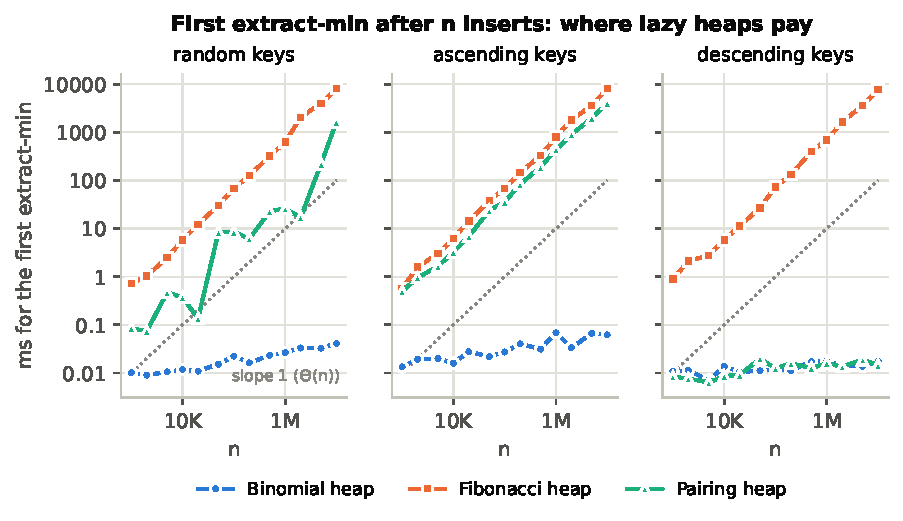
\includegraphics[width=\linewidth]{figures/first_extract_min.pdf}
  \caption{Time of the first extract-min after $n$ inserts. The dotted line has slope 1. The lazy heaps pay here for all their cheap inserts; the binomial heap was tidy all along.}
  \label{fig:first}
\end{figure}

Figure~\ref{fig:first} shows the cost that amortization hides. After $n$
inserts the Fibonacci heap has $n$ one-node trees, and its first extract-min
consolidates all of them: slope 1.03--1.06 in every key order, and 8.1\,s at
$n = 10^7$. The pairing heap behaves as its structure predicts. After ascending
inserts the root has $n-1$ children, which the first extract-min must pair
(slope 1.03; 4.0\,s). After descending inserts every new key is a new minimum,
so the heap is a path and the first extract-min costs 0.01\,ms. With random
keys the root holds only the items inserted after the minimum, so the cost is
erratic, but it still grows linearly (slope 1.08). The binomial heap stays
below 0.07\,ms throughout, as its $O(\log n)$ worst case requires. The pairing
heap keeps paying after the first call: its warm-up batch costs 87.8\us{} per
extract-min, five times its steady state, while the warm-up of the other two
heaps matches their steady state. This supports the analysis: the lazy heaps
pay for their $O(1)$ inserts later.

\subsection{Extract-Min in Steady State}

\begin{figure}[t]
  \centering
  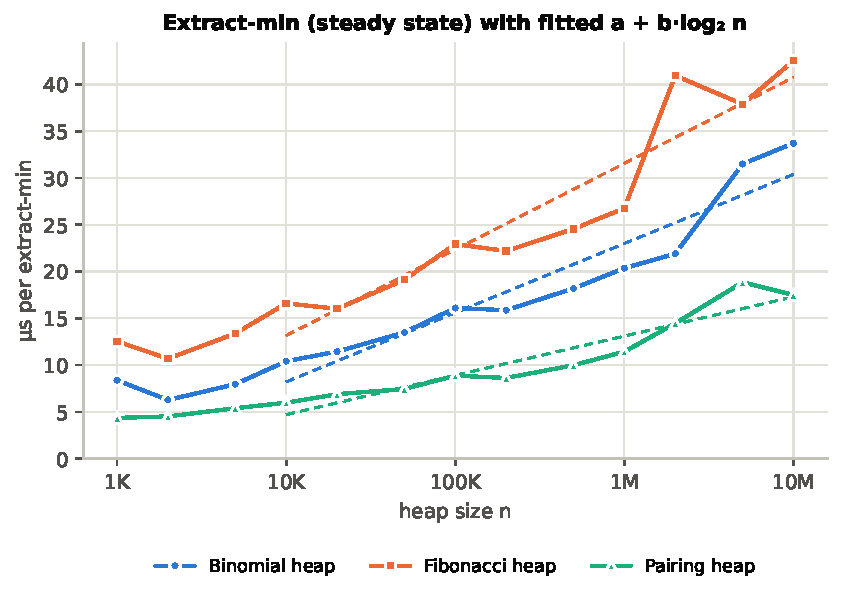
\includegraphics[width=0.75\linewidth]{figures/extract_min_time.pdf}
  \caption{Steady-state extract-min with fitted $a + b\log_2 n$ curves (dashed, $n \ge 10^4$). The cost grows faster than $\log n$ once the heap outgrows the caches.}
  \label{fig:extract}
\end{figure}

Figure~\ref{fig:extract} confirms the ranking reported by Larkin et
al.~\cite{larkin2014}: the pairing heap is fastest (17.5\us{} at $10^7$),
ahead of the binomial (33.7\us) and Fibonacci (42.5\us) heaps. The growth is
only partly logarithmic. From $n = 10^3$ to $10^7$, $\log_2 n$ grows by a factor
of 2.3, but the cost grows by 3.4--4.0 times. The $a + b\log_2 n$ fits reach
only $R^2 = 0.88$--$0.90$, with negative intercepts: the cost per level rises
with the heap's size. From $10^6$ items on, each heap occupies more than
100\,MB, far beyond the 24\,MB L3 cache, so nearly every node visit can miss the
cache. Larkin et al.\ found the wall-clock time of heaps to be strongly
correlated with the L1 cache miss rate~\cite{larkin2014}. We did not measure
cache misses directly, so this is an explanation consistent with the data
rather than a proof. The operation count
is still $O(\log n)$; what grows is the cost of each pointer it follows.

\subsection{Decrease-Key and Its Deferred Cost}

\begin{figure}[t]
  \centering
  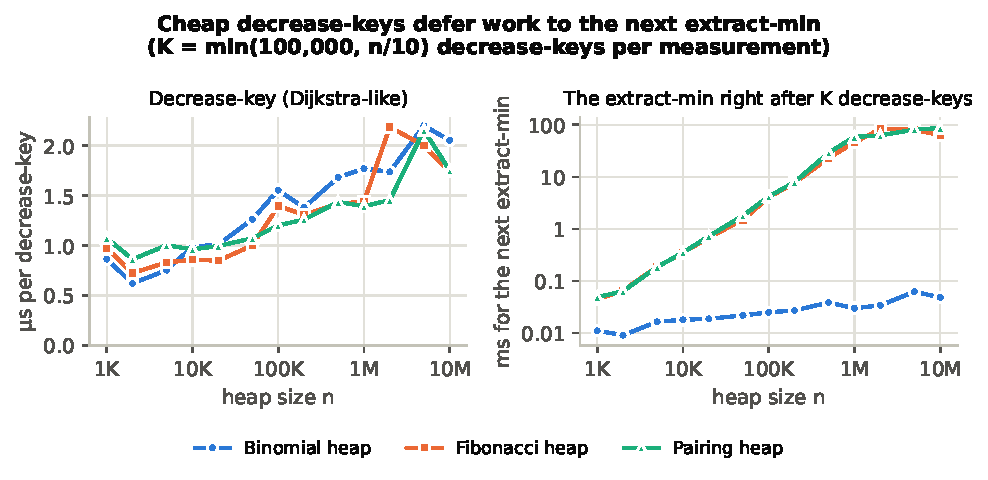
\includegraphics[width=\linewidth]{figures/decrease_key_time.pdf}
  \caption{Left: cost of a Dijkstra-like decrease-key. Right: the single extract-min that follows $K$ of them. The lazy heaps' decrease-keys are cheap because their cost moves into the next extract-min.}
  \label{fig:decrease}
\end{figure}

When every decreased key becomes the new minimum, the decrease-key path of the
binomial heap reaches the root. It then costs 9.74\us{} at $10^7$ (slope 0.21),
against 2.37 and 1.90\us{} for the Fibonacci and pairing heaps (slopes 0.10 and
0.11): $O(\log n)$ against $O(1)$, as predicted. With Dijkstra-like keys,
which land between the current minimum and the old key, all three heaps cost
about 2\us{} (Figure~\ref{fig:decrease}, left). A binomial bubble-up stops as
soon as heap order is restored, which for such keys is usually well before the
root, as the gap between 2.05 and 9.74\us{} suggests. The right panel shows where the lazy heaps'
savings go. After $10^5$ Dijkstra-like decrease-keys, the next extract-min
takes 63\,ms (Fibonacci) and 86\,ms (pairing), against 0.05\,ms for the
binomial heap, because the lazy heaps must re-link the $10^5$ subtrees they cut
out. The panel grows with $n$ until $K$ reaches its cap of $10^5$ at
$n = 10^6$, then flattens. When the keys go to new minima, the pairing heap
builds a chain and its next extract-min costs only 0.01\,ms, while the
Fibonacci heap must consolidate $10^5$ new roots (139\,ms).

\subsection{Merge}

\begin{figure}[t]
  \centering
  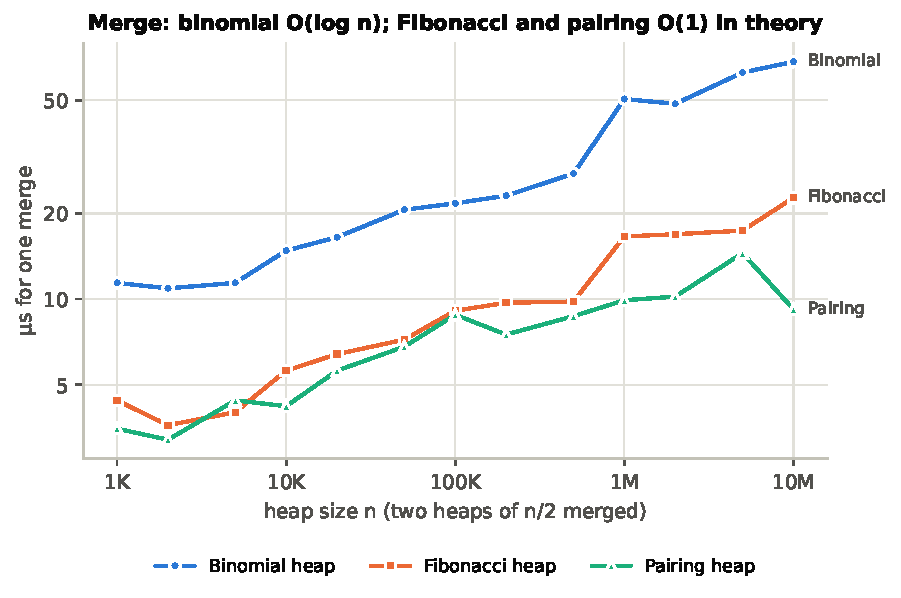
\includegraphics[width=0.75\linewidth]{figures/merge_time.pdf}
  \caption{One merge of two heaps of $n/2$ items. The binomial merge grows with $\log n$. The $O(1)$ merges do constant work but still slow down as the heaps grow.}
  \label{fig:merge}
\end{figure}

The binomial merge grows from 11.4\us{} at $n = 10^3$ to 68.3\us{} at $10^7$
(Figure~\ref{fig:merge}), as expected for an operation that walks
$O(\log n)$ roots. The Fibonacci and pairing merges perform a fixed number of
pointer updates, yet they slow down from 4.4 to 22.7\us{} and from 3.5 to
9.2\us{}. This contradicts a literal reading of $O(1)$. The work is constant,
but a single merge touches roots that were last used long before, while the
other $n$ nodes were being built. In a large heap those roots are no longer in
the CPU cache, so every pointer access waits for main memory. Single-operation
timings are also noisy: they are medians of three runs only up to
$10^6$.

\subsection{Dijkstra's Algorithm}

\begin{figure}[t]
  \centering
  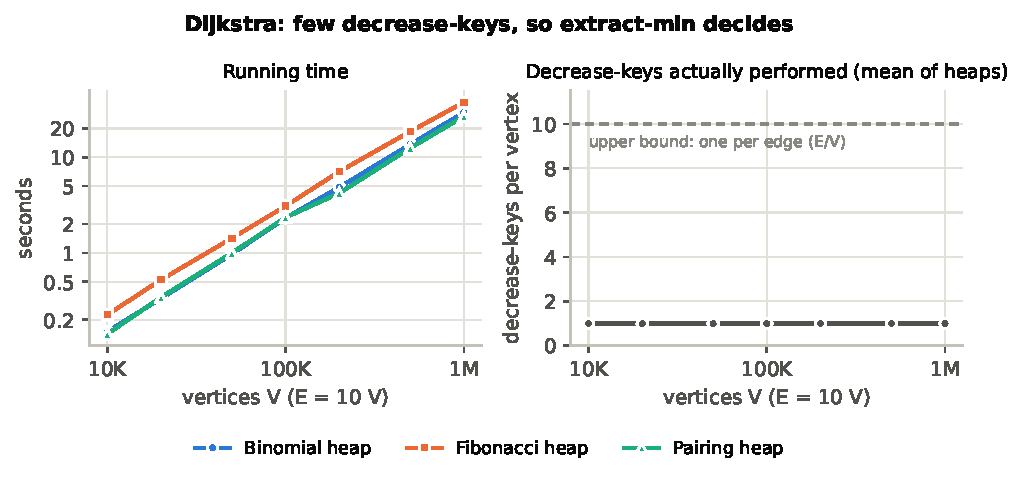
\includegraphics[width=\linewidth]{figures/dijkstra_time.pdf}
  \caption{Dijkstra's algorithm on graphs with $E = 10V$. Left: running time. Right: decrease-keys per vertex, about one, against the upper bound of ten (one per edge).}
  \label{fig:dijkstra}
\end{figure}

All three heaps return identical distances on every graph. At $V = 10^6$ the
pairing heap takes 26.8\,s, the binomial heap 29.3\,s and the Fibonacci heap
37.5\,s (Figure~\ref{fig:dijkstra}). This \emph{contradicts} the ranking by
worst-case bound, in which the Fibonacci heap's $O(E + V\log V)$ beats the
others' $O((V+E)\log V)$. The right panel explains the result: only 0.99
decrease-keys per vertex occur (993,926--993,971 at $V = 10^6$), far below
the possible $E/V = 10$. This is consistent with the
$O(V\log(1+E/V))$ expectation of Goldberg and Tarjan~\cite{goldberg1996}. The
Fibonacci heap's $O(1)$ decrease-key therefore has little to save, while every
vertex pays for its slower extract-min. The running times grow with slopes
1.11--1.15, slightly above 1, in line with the $\log V$ factor and the
cache effects above.

%% ---------------------------------------------------------------------------
\section{Discussion}
\label{sec:discussion}

\textbf{The analysis predicts the shapes.} Every growth rate the analysis
predicts appears in the data:
\begin{itemize}
  \item constant inserts and finds;
  \item linear first extract-mins for the lazy heaps and logarithmic ones for the binomial heap;
  \item $O(1)$ against $O(\log n)$ decrease-keys when keys move to the root;
  \item the deferred cost of laziness, which shows up in the next extract-min.
\end{itemize}
The two departures, extract-min growing faster than $\log n$ and the
$O(1)$ merges slowing down, come from the memory hierarchy, which the RAM
model ignores, not from extra operations.

\textbf{The constants decide the ranking.} Asymptotic bounds say nothing about
constant factors, and the constants reverse the textbook order for Dijkstra's
algorithm. A rough budget shows why. At $V = 10^6$ the run performs $10^6$
extract-mins and about $10^6$ decrease-keys. At about 2\us{} each, all the
decrease-keys together cost about 2\,s, so even a free decrease-key could save
at most 2\,s of the 27--38\,s total. Extract-min, by contrast, is 2.4 times
slower in the Fibonacci heap than in the pairing heap at $10^7$ items. Three
features make it slower: a larger node (8 fields against 5), consolidation
through a degree table over circular lists, and mark bookkeeping. This agrees
with Larkin et al., who found that ``pairing heaps dominate Fibonacci heaps
across the board''~\cite{larkin2014}.

\textbf{Which heap to use.}
\begin{itemize}
  \item The \emph{pairing heap} is the best default: it is the fastest in steady state and in Dijkstra's algorithm, and the smallest. Its cost is a warm-up after bulk inserts or merges. GCC also makes it the default~\cite{gccpbds}.
  \item The \emph{binomial heap} never has a slow operation (at most 0.07\,ms for any first extract-min, against seconds for the lazy heaps). This suits latency-sensitive uses where one slow operation is worse than a slightly higher average.
  \item The \emph{Fibonacci heap} is mainly of theoretical value. It pays off only when decrease-keys greatly outnumber extract-mins, which random sparse graphs do not provide.
\end{itemize}

\textbf{Threats to validity.}
\begin{itemize}
  \item CPython's interpretive overhead inflates every constant. It probably affects the three heaps similarly, but a compiled implementation could rank them differently.
  \item All measurements come from one machine.
  \item Sizes above $10^6$ were measured once.
  \item Pausing the garbage collector removes collection pauses that a real application would experience.
\end{itemize}

%% ---------------------------------------------------------------------------
\section{Conclusion}

We implemented, analysed and benchmarked the binomial, Fibonacci and pairing
heaps on up to ten million items. The measurements support the amortized
analysis wherever it makes a prediction about growth, including the expensive
operations that amortization hides. They also show that the best worst-case
bound does not give the fastest program. On Dijkstra's algorithm the Fibonacci
heap is the slowest of the three, because decrease-keys are rare and its
extract-min is expensive. The pairing heap, whose analysis is still open, is
the fastest in practice.

%% ---------------------------------------------------------------------------
\section*{Use of Generative AI}

This work was produced with the assistance of Claude Code (Anthropic, Claude
Opus 5.5), as allowed by the course policy with disclosure.
\begin{itemize}
  \item \textbf{The assistant} wrote the plan, the three heap implementations, Dijkstra's algorithm, the dataset, benchmark and plotting scripts, the demo and the unit tests, and drafted this report except Section~\ref{sec:why}.
  \item \textbf{The author}
  \begin{itemize}
    \item chose the data structures and the application;
    \item directed the work in twelve phases, and reviewed and ran each phase's code and tests before it was committed;
    \item approved the design decisions recorded in the repository's \code{docs/review\_log.md} (for example, timing Dijkstra-like decrease-keys and separating the warm-up from the steady state);
    \item published the dataset;
    \item wrote Section~\ref{sec:why}.
  \end{itemize}
\end{itemize}

\bibliographystyle{ACM-Reference-Format}
\bibliography{references}

\end{document}
